% Completed CPU results; companion GPU results are in supplementary_gpu_results.tex.
% Sources: results/revision_c3/exports and native_budget_audit.
\subsection{Structural retention results and compression trade-offs}

The primary CPU study completed 620 dataset/split/variant summaries, with a
further 60 summaries from the native-implementation budget audit. All native
edge sets were reproduced exactly at their archived budgets on validation and
test. Alternative selectors preserved candidate order and satisfied the matched
unique-edge budgets. These summaries reuse 2,100 validation and 2,100 test rows;
they are not independent new datasets or examples.

\paragraph{Duplicate removal is distinct from unique-edge removal.}
PrimeKG source graphs contain a mean of 59.932 edge occurrences but only 38.094
unique triples per test row. The original fuzzy output retains 32.340 unique
triples. Thus, the mean reduction of 27.592 occurrences consists of 21.838
duplicate occurrences and 5.754 unique triples. Approximately 79.1\% of the
aggregate count reduction is attributable to duplicate removal. The other four
datasets have no such source duplicates in these prepared test inputs. This is
a counting decomposition, not a claim that duplicates have no computational
effect: the encoder can process repeated triples as repeated messages.

\begin{table}[t]
\centering\small
\caption{Matched-budget test retention of candidate--query reachability within
three edges. Coverage is relative to source-covered candidates. Random reports
mean $\pm$ standard deviation over all five seeds, not a confidence interval.
$N$ counts rows with at least one reachable source candidate.}
\label{tab:c3-reachability}
\begin{tabular}{lrrrrr}
\hline
Dataset & $N$ & Fuzzy coverage & Fuzzy reachability & Random & Shortest paths \\
\hline
PrimeKG & 488 & 1.0000 & 0.7737 & $0.7760\pm0.0038$ & 0.9985 \\
PharmKG & 500 & 1.0000 & 0.9010 & $0.4423\pm0.0064$ & 1.0000 \\
Hetionet & 90 & 1.0000 & 0.4835 & $0.4848\pm0.0428$ & 1.0000 \\
DRKG & 386 & 1.0000 & 0.8921 & $0.5043\pm0.0170$ & 1.0000 \\
repoDB & 297 & 1.0000 & 0.9546 & $0.5465\pm0.0241$ & 1.0000 \\
\hline
\end{tabular}
\end{table}

\paragraph{Coverage does not imply path preservation.}
Although original fuzzy retrieval preserves relative candidate coverage on all
five datasets, its reachability retention varies substantially
(Table~\ref{tab:c3-reachability}). Fuzzy retrieval preserves substantially more
reachability than uniform random selection on PharmKG, DRKG, and repoDB, whereas
the PrimeKG and Hetionet point estimates are similar to random. The joint
query-cluster/seed bootstrap interval for random minus fuzzy reachability is
$[-0.4829,-0.4337]$ on PharmKG. The corresponding intervals are
$[-0.4433,-0.3353]$ on DRKG and $[-0.4492,-0.3661]$ on repoDB;
the PrimeKG and Hetionet intervals include zero. These are exploratory,
unadjusted intervals.

The shortest-path baseline retains nearly all source-reachable candidates at
the same edge count. This is partly aligned with its explicit selection
objective and does not establish semantic superiority. It also trades away
coverage of other candidates: relative candidate coverage is 0.8514 on
Hetionet, 0.8199 on DRKG, and 0.8971 on repoDB, compared with 1.0000 for original
fuzzy retrieval. Thus, preserving candidate incidence and preserving connected
query--candidate paths are different selection goals.

\begin{table}[t]
\centering\small
\caption{Retention of exact edge-labeled simple paths of length three at
matched budgets. $N$ is the number of rows containing at least one such source
path; rows without source paths are undefined and excluded. These paths are
structural witnesses, not validated therapeutic mechanisms.}
\label{tab:c3-path-witnesses}
\begin{tabular}{lrrrr}
\hline
Dataset & $N$ & Original fuzzy & Random (five seeds) & Shortest paths \\
\hline
PrimeKG & 488 & 0.6543 & $0.6443\pm0.0047$ & 0.8199 \\
PharmKG & 31 & 0.0000 & $0.1801\pm0.0967$ & 0.8604 \\
Hetionet & 64 & 0.0000 & $0.1615\pm0.0589$ & 0.6207 \\
DRKG & 201 & 0.4767 & $0.1629\pm0.0078$ & 0.6496 \\
repoDB & 219 & 0.5286 & $0.1552\pm0.0185$ & 0.8322 \\
\hline
\end{tabular}
\end{table}

Length-three path retention exposes additional losses that are hidden by
coverage alone (Table~\ref{tab:c3-path-witnesses}). Original fuzzy retrieval
retains no such witnesses in the eligible PharmKG and Hetionet rows. This does
not mean that every row loses all connectivity: only 31 PharmKG rows have a
length-three source witness, and shorter paths can remain. Conversely,
original fuzzy retrieval retains more length-three witnesses than random on
DRKG and repoDB. The full relation-distribution, rank-band, incoming-context,
gene-annotation, and gold-conditional diagnostics are supplied in the result
workbook rather than collapsed into a single information-retention score.

\paragraph{Source availability and annotated paths.}
Fuzzy outputs contain the query node in 100\%, 96.8\%, 100\%, 84.8\%, and
59.4\% of test rows on PrimeKG, PharmKG, Hetionet, DRKG, and repoDB,
respectively. Conditional reachability retention must be interpreted with its
source eligibility rather than as a fraction of every test row. The additional
Gene-intermediate diagnostic pools length-two and length-three witnesses with
explicitly annotated intermediate nodes: fuzzy retention is 1.0000 on the
31 eligible Hetionet rows and 0.9366 on the 243 eligible DRKG rows. These small,
annotation-dependent subsets do not establish general mechanism preservation.
In particular, the Hetionet value does not contradict the loss of its separate
length-three witness set. PrimeKG and PharmKG types are unavailable to this
audit; repoDB has no eligible source Gene-intermediate witnesses.

\paragraph{Budget feasibility and operating curves.}
The native replay audit confirms that the original PrimeKG coverage-first
implementation can exceed a newly imposed small target. At a requested budget
of 20\% of unique source edges, its mean requested/actual counts are
7.576/15.662, and 99.8\% of test rows exceed the request. At 35\%, the counts are
13.336/15.886 and the excess rate is 74.2\%. No excess occurs at the archived
native budgets used in the matched comparison. We report these native-policy
points separately from strict-budget controls. Operating curves must therefore
identify the selector and distinguish requested budget from actual graph size.

\begin{figure}[p]
\centering
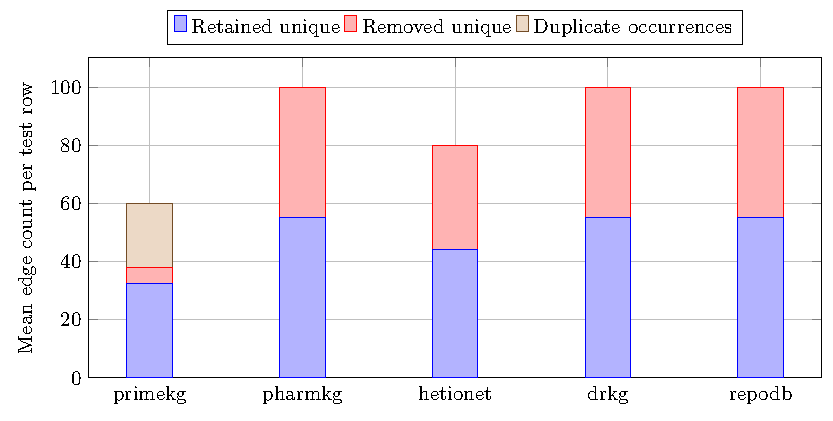
\includegraphics[width=.96\textwidth]{../../results/revision_c3/exports/compression_decomposition.pdf}
\caption{Decomposition of source edge occurrences into retained unique triples,
removed unique triples, and duplicate occurrences. Counts are means over test
rows; duplicate removal is separated from structural edge loss.}
\label{fig:c3-duplicates}
\end{figure}

\begin{figure}[p]
\centering
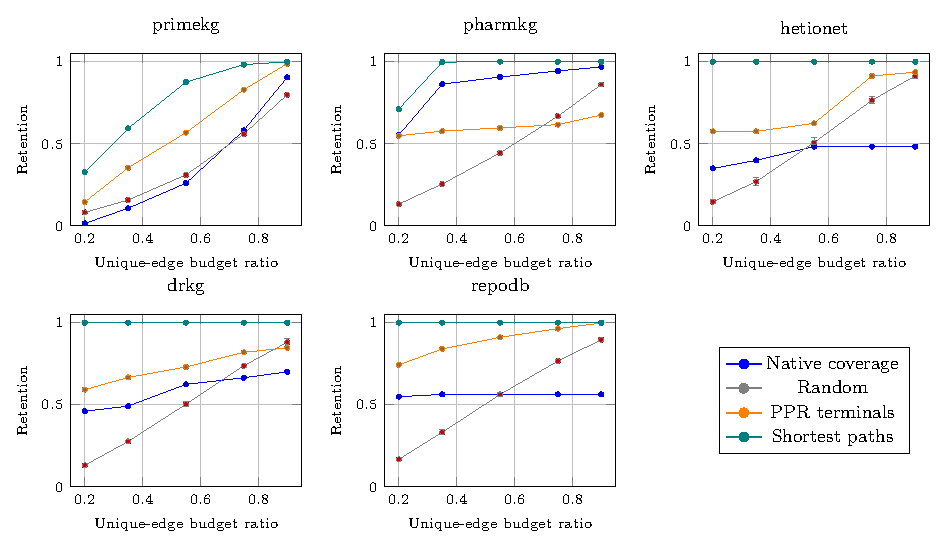
\includegraphics[width=.98\textwidth]{../../results/revision_c3/exports/budget_reach3_retention.pdf}
\caption{Candidate--query reachability retention for strict-budget selectors.
The native-score coverage control is distinguished from the original
dataset-specific selector. Random error bars show seed variability, not test
confidence intervals. Native implementation budget violations are reported
separately in the audit tables.}
\label{fig:c3-budget-reach}
\end{figure}

\begin{figure}[p]
\centering
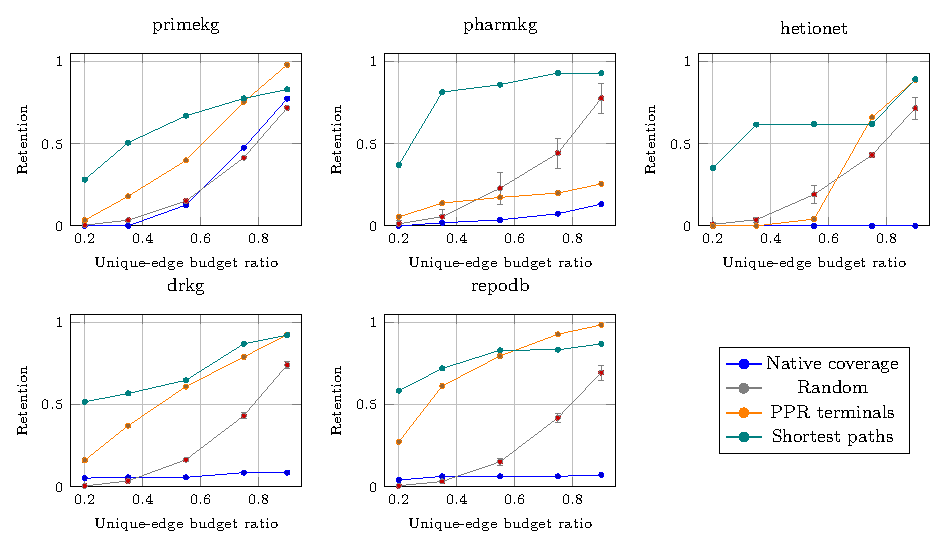
\includegraphics[width=.98\textwidth]{../../results/revision_c3/exports/budget_path3_retention.pdf}
\caption{Exact length-three path-witness retention under the same strict-budget
controls. Means exclude queries without a corresponding source witness;
eligible counts are provided in the accompanying tables.}
\label{fig:c3-budget-paths}
\end{figure}
